%!TEX TS-program = xelatex

% HSE Beamer Theme
% by Danil Fedorovykh
% http://hse.ru/staff/df
%
% Version 2.0 (English)
% January 2022

%%% Set up the free HSE Sans font
%%% https://www.hse.ru/info/brandbook/#font

\documentclass[aspectratio=169]{beamer}

\newbool{russian}
\booltrue{russian} % Uncomment if in Russian
\usepackage{HSE-theme/beamerthemeHSE} % Load HSE theme
\usepackage[no-math]{fontspec}      % fonts loading
\usepackage{caption}
\usepackage{subfigure}
\usepackage{subcaption}
\usepackage{hyperref}
\usepackage[dvipsnames]{xcolor}
\usepackage{ragged2e}
\captionsetup[figure]{labelformat=empty}
\captionsetup[subfigure]{labelformat=empty}
\renewcommand*{\thesubfigure}{(\arabic{subfigure})}
\setsansfont{HSE Sans}
%\graphicspath{{./images/}}
\graphicspath{{/home/llyy/Yandex.Disk/personal/knowledge/general/algorithms_course/repo/algorithms_course/1_arrays_complexity_testing/lection/images}}


%%% Информация об авторе и выступлении
\title[Title]{Алгоритмы и структуры данных} 
\subtitle{Лекция 1. Массивы, вычислительная сложность, тестирование}
\author[Author's name]{Илья Сергеевич Бычков\\ \smallskip \scriptsize \url{ibychkov@hse.ru}}
\institute{НИУ ВШЭ - Нижний Новгород}
\date{\today}


\begin{document}

\frame[plain]{\titlepage}


%%%%%%%%%%%%%%%%%%%%%%%%%%%%%%%%%%%%%%%%%%%%%%%%%%%%%%%%%%%%%%%%%%%%%%%%%%%%%%%%%%%%%%%%%%%%%%%%%%
\begin{frame}
\frametitle{Повторение}
\framesubtitle{Вопросы}
Алгоритм, программа\newline\newline
Вычислительные машины\newline\newline
Языки программирования\newline\newline
Трансляция\newline\newline
Данные, системы счисления, память\newline\newline
Представление данных \newline\newline
Битовые операции\newline\newline
\end{frame}

%%%%%%%%%%%%%%%%%%%%%%%%%%%%%%%%%%%%%%%%%%%%%%%%%%%%%%%%%%%%%%%%%%%%%%%%%%%%%%%%%%%%%%%%%%%%%%%%%%
\begin{frame}[c]
%\frametitle{A first slide}

\begin{center}
\Huge Лекция 1.

\Huge Массивы, вычислительная сложность, тестирование
\end{center}

\end{frame}

%%%%%%%%%%%%%%%%%%%%%%%%%%%%%%%%%%%%%%%%%%%%%%%%%%%%%%%%%%%%%%%%%%%%%%%%%%%%%%%%%%%%%%%%%%%%%%%%%%
\begin{frame}
\frametitle{Массивы, вычислительная сложность, тестирование}
\framesubtitle{План лекции}

\begin{enumerate}
  \setcounter{enumi}{-1}
  \item{План лекции}
  \item{\textcolor{blue}{Структура данных массив}}
  \item{Вычислительные задачи и корректность алгоритмов}
  \item{Вычислительная сложность алгоритмов}
  \item{Тестирование программ}
\end{enumerate}
\end{frame}



%%%%%%%%%%%%%%%%%%%%%%%%%%%%%%%%%%%%%%%%%%%%%%%%%%%%%%%%%%%%%%%%%%%%%%%%%%%%%%%%%%%%%%%%%%%%%%%%%%
\begin{frame}
\frametitle{Структура данных: массив}
\framesubtitle{Структура данных}
\justifying

В большинстве случаев объем данных, обрабатываемых алгоритмам, достаточно велик, что не позволяет ограничиваться только использованием \textcolor{red}{переменных} (если конечно вы не решаете только задачи типа “A+B Problem”).\newline\newline
В таких случаях на помощь приходят разнообразные \textcolor{red}{структуры данных}.\newline\newline
\textcolor{red}{Структура данных} — это контейнер, который хранит данные и обеспечивает работу с ними в соответствии с определенными правилами.\newline\newline
Первая и самая простая структура данных (часто ее даже не относят к структурам данных), которую мы рассмотрим, называется \textcolor{red}{массив}.\newline\newline


\end{frame}

%%%%%%%%%%%%%%%%%%%%%%%%%%%%%%%%%%%%%%%%%%%%%%%%%%%%%%%%%%%%%%%%%%%%%%%%%%%%%%%%%%%%%%%%%%%%%%%%%%
\begin{frame}
\frametitle{Структура данных: массив}
\framesubtitle{Массив}
\justifying
\textcolor{red}{Массив} - это структура данных, для которой характерно:
\begin{enumerate}
  \item{Хранение элементов одного типа}
  \item{Размещение элементов последовательно в памяти}
  \item{Единое имя для всех элементов\newline}
\end{enumerate}
Полезно думать о массиве как об определенном наборе переменных одного типа.
\begin{figure}
    \captionsetup[subfigure]{labelformat=empty}
    \centering
    \subfigure[{ \scriptsize Введение в массивы, Источник - \href{https://www.geeksforgeeks.org/introduction-to-arrays-data-structure-and-algorithm-tutorials/}{GeeksForGeeks} }]{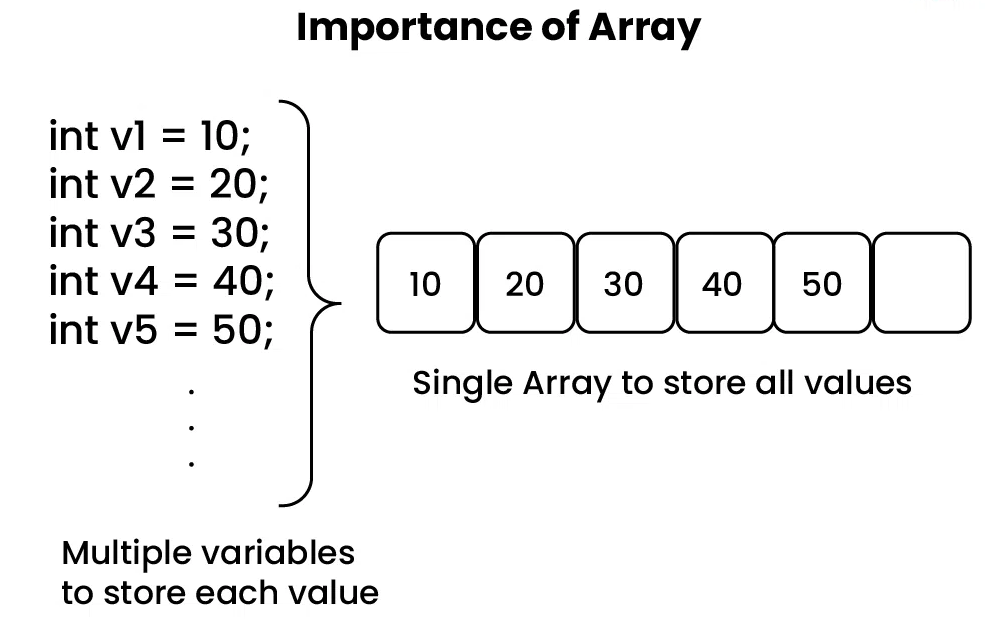
\includegraphics[width=65mm, height=35mm]{array_intro}} 
\end{figure}
\end{frame}

%%%%%%%%%%%%%%%%%%%%%%%%%%%%%%%%%%%%%%%%%%%%%%%%%%%%%%%%%%%%%%%%%%%%%%%%%%%%%%%%%%%%%%%%%%%%%%%%%%
\begin{frame}
\frametitle{Структура данных: массив}
\framesubtitle{Устройство массива}
\justifying
\small
\textcolor{red}{Имя массива} указывает на \textcolor{red}{адрес} в памяти его самого первого элемента. \newline\newline Доступ к элементам массива осуществляется с помощью \textcolor{red}{индексов} или \textcolor{red}{смещений}. \newline\newline
Самый первый элемент имеет \textcolor{red}{нулевое смещение} относительно адреса массива в памяти.\newline\newline
Каждый элемент массива имеет свой адрес и занимает одинаковое и фиксированное число байт, которое зависит от типа данных.

\begin{figure}
    \captionsetup[subfigure]{labelformat=empty}
    \centering
    \subfigure[{ \scriptsize Строение массива, Источник - \href{https://www.geeksforgeeks.org/introduction-to-arrays-data-structure-and-algorithm-tutorials/}{GeeksForGeeks} }]{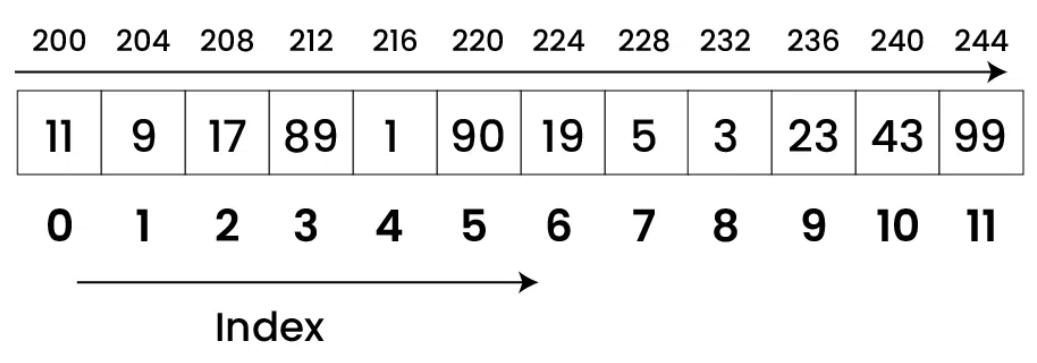
\includegraphics[width=85mm, height=30mm]{array_structure}} 
\end{figure}
\end{frame}

%%%%%%%%%%%%%%%%%%%%%%%%%%%%%%%%%%%%%%%%%%%%%%%%%%%%%%%%%%%%%%%%%%%%%%%%%%%%%%%%%%%%%%%%%%%%%%%%%%
\begin{frame}
\frametitle{Структура данных: массив}
\framesubtitle{Типы массивов}
\justifying
\small
\begin{figure}
    \captionsetup[subfigure]{labelformat=empty}
    \centering
    \subfigure[{ \scriptsize Типы массивов, Источник - \href{https://www.geeksforgeeks.org/introduction-to-arrays-data-structure-and-algorithm-tutorials/}{GeeksForGeeks} }]{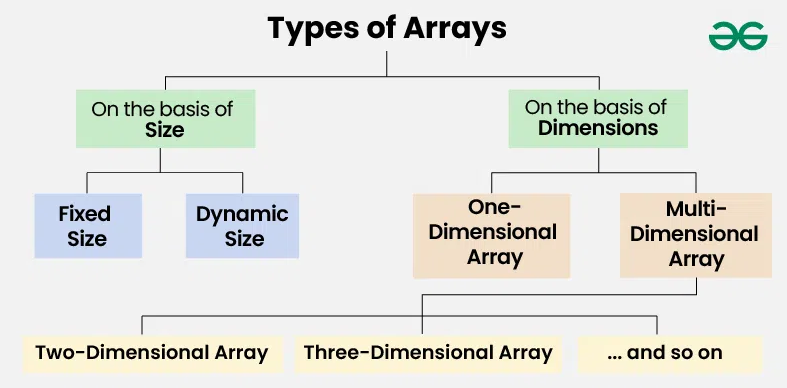
\includegraphics[width=95mm, height=50mm]{array_types}} 
\end{figure}
\end{frame}

%%%%%%%%%%%%%%%%%%%%%%%%%%%%%%%%%%%%%%%%%%%%%%%%%%%%%%%%%%%%%%%%%%%%%%%%%%%%%%%%%%%%%%%%%%%%%%%%%%
\begin{frame}
\frametitle{Структура данных: массив}
\framesubtitle{Алгоритмы на массивах}
\justifying
\small
Операции для прямой модификации массивов:
\begin{itemize}
  \item{замена элемента/добавление в конец}
  \item{вставка элемента на выбранную позицию}
  \item{удаление элемента на выбранной позиции\newline}
\end{itemize}

Алгоритмы на массивах:
\begin{itemize}
  \item{поиск элемента с заданными свойствами}
  \item{сортировка массива}
\end{itemize}
\end{frame}

%%%%%%%%%%%%%%%%%%%%%%%%%%%%%%%%%%%%%%%%%%%%%%%%%%%%%%%%%%%%%%%%%%%%%%%%%%%%%%%%%%%%%%%%%%%%%%%%%%
\begin{frame}
\frametitle{Структура данных: массив}
\framesubtitle{Доступ к элементам}
\justifying
\small
Благодаря своей природе массив обладает эффективным \textcolor{red}{произвольным доступом (random access)} к данным. Любой элемент массива может быть считан или перезаписан за фиксированное число операций, которое не зависит от размера массива. Это называется \textcolor{red}{константной сложностью} и записывается как \textcolor{red}{O(1)}.\newline
\begin{figure}
    \captionsetup[subfigure]{labelformat=empty}
    \centering
    \subfigure[{ \scriptsize Доступ к элементам массива, Источник - \href{https://www.geeksforgeeks.org/introduction-to-arrays-data-structure-and-algorithm-tutorials/}{GeeksForGeeks} }]{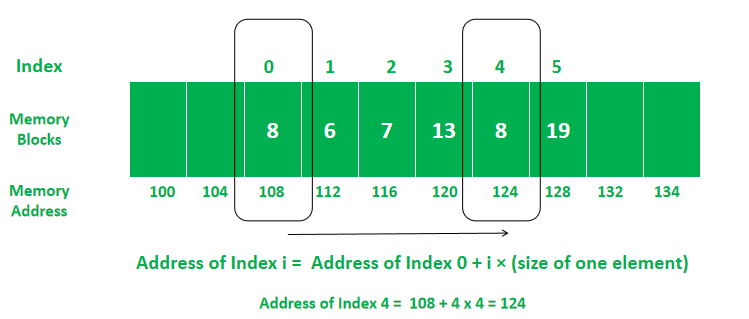
\includegraphics[width=100mm, height=43mm]{array_access}} 
\end{figure}
\end{frame}

%%%%%%%%%%%%%%%%%%%%%%%%%%%%%%%%%%%%%%%%%%%%%%%%%%%%%%%%%%%%%%%%%%%%%%%%%%%%%%%%%%%%%%%%%%%%%%%%%%
\begin{frame}
\frametitle{Структура данных: массив}
\framesubtitle{Замена элемента/добавление в конец}
\justifying
\small
Рисуем на доске
\end{frame}

%%%%%%%%%%%%%%%%%%%%%%%%%%%%%%%%%%%%%%%%%%%%%%%%%%%%%%%%%%%%%%%%%%%%%%%%%%%%%%%%%%%%%%%%%%%%%%%%%%
\begin{frame}
\frametitle{Структура данных: массив}
\framesubtitle{Вставка элемента}
\justifying
\small
\textcolor{blue}{Входные данные:} массив, элемент для вставки, позиция для вставки\newline
\textcolor{blue}{Результат:} массив с вставленным элементов\newline
\textcolor{blue}{Время операции:} в худшем случае линейное по количеству элементов, O(n)
\begin{figure}
    \captionsetup[subfigure]{labelformat=empty}
    \centering
    \subfigure[{ \scriptsize Вставка в массив, Источник - \href{https://www.w3resource.com/java-exercises/array/java-array-exercise-9.php}{w3resource} }]{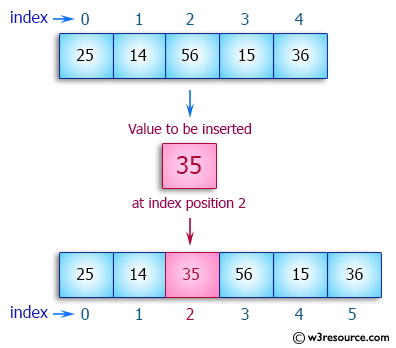
\includegraphics[width=70mm, height=53mm]{array_insert}} 
\end{figure}
\end{frame}

%%%%%%%%%%%%%%%%%%%%%%%%%%%%%%%%%%%%%%%%%%%%%%%%%%%%%%%%%%%%%%%%%%%%%%%%%%%%%%%%%%%%%%%%%%%%%%%%%%
\begin{frame}
\frametitle{Структура данных: массив}
\framesubtitle{Удаление элемента}
\justifying
\small
\textcolor{blue}{Входные данные:} массив, позиция удаляемого элемента \newline
\textcolor{blue}{Результат:} массив без удаленного элемента\newline
\textcolor{blue}{Время операции:} в худшем случае линейное по количеству элементов, O(n)
\begin{figure}
    \captionsetup[subfigure]{labelformat=empty}
    \centering
    \subfigure[{ \scriptsize Удаление из массива, Источник - неизвестен}]{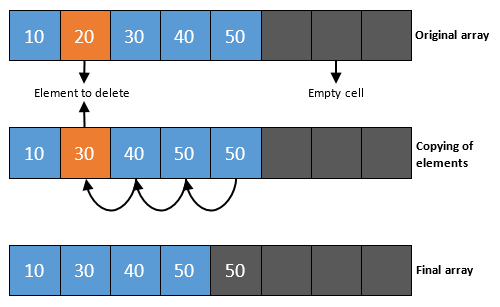
\includegraphics[width=80mm, height=50mm]{array_remove}} 
\end{figure}
\end{frame}

%%%%%%%%%%%%%%%%%%%%%%%%%%%%%%%%%%%%%%%%%%%%%%%%%%%%%%%%%%%%%%%%%%%%%%%%%%%%%%%%%%%%%%%%%%%%%%%%%%
\begin{frame}
\frametitle{Структура данных: массив}
\framesubtitle{Поиск элемента/элементов с заданными свойствами}
\justifying
\small
\textcolor{blue}{Входные данные:} массив, искомый элемент или критерий(функция) \newline
\textcolor{blue}{Результат:} индекс или набор индексов искомых элементов\newline
\textcolor{blue}{Время операции:} в худшем случае линейное по количеству элементов, O(n)
\begin{figure}
    \captionsetup[subfigure]{labelformat=empty}
    \centering
    \subfigure[{ \scriptsize Поиск в массиве, Источник - \href{https://www.geeksforgeeks.org/linear-search/}{GeeksForGeeks}}]{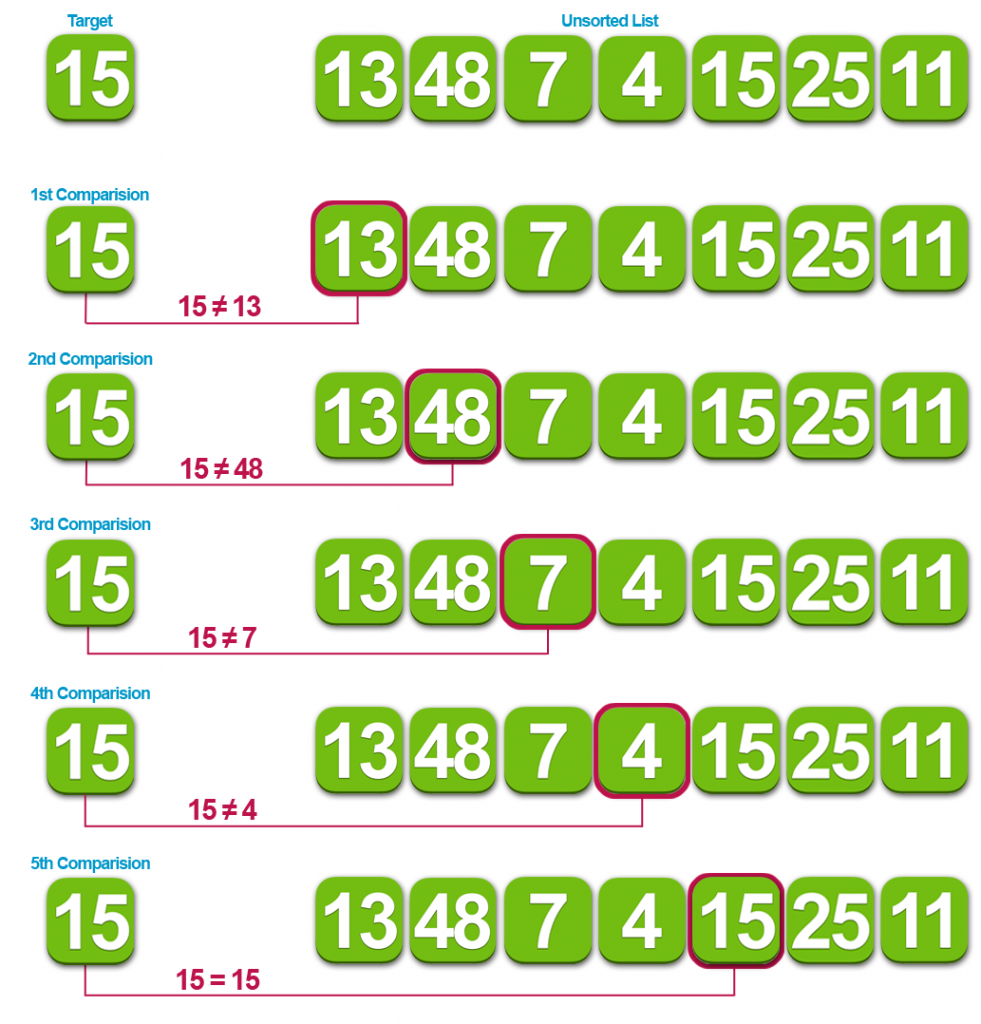
\includegraphics[width=60mm, height=50mm]{array_search}}
\end{figure}
\end{frame}

%%%%%%%%%%%%%%%%%%%%%%%%%%%%%%%%%%%%%%%%%%%%%%%%%%%%%%%%%%%%%%%%%%%%%%%%%%%%%%%%%%%%%%%%%%%%%%%%%%
\begin{frame}
\frametitle{Структура данных: массив}
\framesubtitle{Многомерные массивы}
\justifying
\small
\textcolor{red}{Многомерные массивы} как правило сохраняют свойство последовательного расположения элементов в памяти.

\begin{figure}
    \captionsetup[subfigure]{labelformat=empty}
    \centering
    \subfigure[{ \scriptsize Многомерные массивы, Источник - неизвестен}]{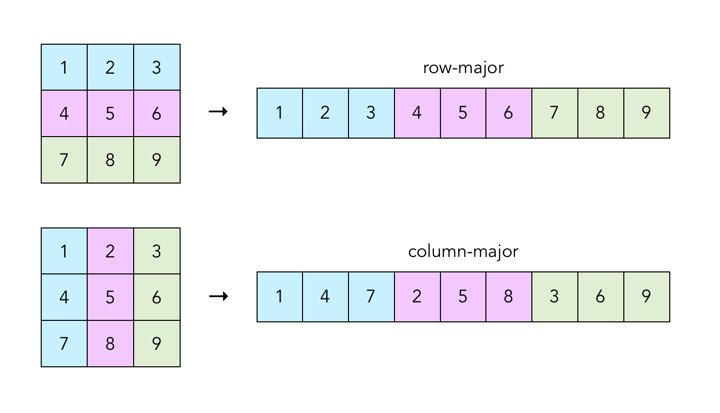
\includegraphics[width=90mm, height=50mm]{array_rowcolumn}} 
\end{figure}
\end{frame}

%%%%%%%%%%%%%%%%%%%%%%%%%%%%%%%%%%%%%%%%%%%%%%%%%%%%%%%%%%%%%%%%%%%%%%%%%%%%%%%%%%%%%%%%%%%%%%%%%%
\begin{frame}
\frametitle{Структура данных: массив}
\framesubtitle{Динамические массивы}
\justifying
\small
Под \textcolor{red}{динамическими массивами} обычно имеют ввиду:

\begin{itemize}
\item{массивы, размер которых не известен заранее, память для них выделяется на этапе работы программы}

\item{структуры данных, имеющих внутри массивы и реализующие специальную логику по автоматическому увеличению их размера при необходимости}
\end{itemize}

\begin{figure}
    \captionsetup[subfigure]{labelformat=empty}
    \centering
    \subfigure[{ \scriptsize Источник - \href{https://en.wikipedia.org/wiki/Dynamic_array}{Wikipedia}}]{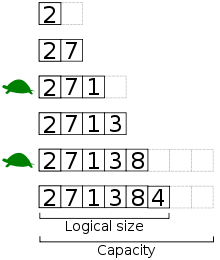
\includegraphics[width=40mm, height=39mm]{array_dynamic}} 
\end{figure}
\end{frame}

%%%%%%%%%%%%%%%%%%%%%%%%%%%%%%%%%%%%%%%%%%%%%%%%%%%%%%%%%%%%%%%%%%%%%%%%%%%%%%%%%%%%%%%%%%%%%%%%%%
\begin{frame}
\frametitle{Структура данных: массив}
\framesubtitle{Динамические массивы}
\justifying
\small

\begin{figure}
    \captionsetup[subfigure]{labelformat=empty}
    \centering
    \subfigure[{ \scriptsize Пример динамического массива, Источник - \href{https://sassafras13.github.io/images/2021-01-16-DynamicResizeLists-fig1.png}{Link}}]{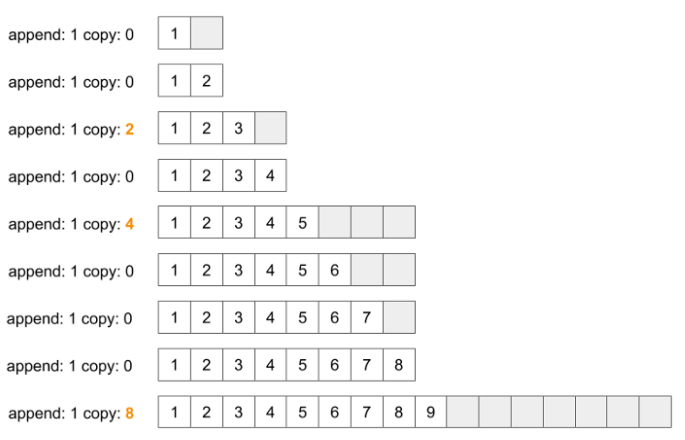
\includegraphics[width=100mm, height=65mm]{array_dynamic_example}} 
\end{figure}
\end{frame}

%%%%%%%%%%%%%%%%%%%%%%%%%%%%%%%%%%%%%%%%%%%%%%%%%%%%%%%%%%%%%%%%%%%%%%%%%%%%%%%%%%%%%%%%%%%%%%%%%%
\begin{frame}
\frametitle{Структура данных: массив}
\framesubtitle{Вычислительная сложность}
\justifying
\small

\begin{figure}
    \captionsetup[subfigure]{labelformat=empty}
    \centering
    \subfigure[{ \scriptsize Вычислительная сложность операций на массивах}]{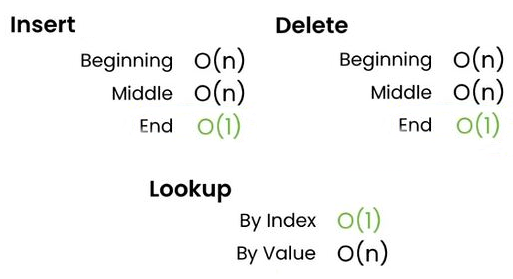
\includegraphics[width=90mm, height=50mm]{array_complexity_table2}} 
\end{figure}
\end{frame}

%%%%%%%%%%%%%%%%%%%%%%%%%%%%%%%%%%%%%%%%%%%%%%%%%%%%%%%%%%%%%%%%%%%%%%%%%%%%%%%%%%%%%%%%%%%%%%%%%%
\begin{frame}
\frametitle{Структура данных: массив}
\framesubtitle{Плюсы и минусы}
\justifying
\small

\begin{figure}
    \captionsetup[subfigure]{labelformat=empty}
    \centering
    \subfigure[{ \scriptsize Достоинства и недостатки массивов}]{
\includegraphics[width=140mm, height=50mm]{array_pros_cons}} 
\end{figure}
\end{frame}

%%%%%%%%%%%%%%%%%%%%%%%%%%%%%%%%%%%%%%%%%%%%%%%%%%%%%%%%%%%%%%%%%%%%%%%%%%%%%%%%%%%%%%%%%%%%%%%%%%
\begin{frame}
\frametitle{Массивы, вычислительная сложность, тестирование}
\framesubtitle{План лекции}

\begin{enumerate}
  \setcounter{enumi}{-1}
  \item{План лекции}
  \item{Структура данных массив}
  \item{\textcolor{blue}{Вычислительные задачи и корректность алгоритмов}}
  \item{Вычислительная сложность алгоритмов}
  \item{Тестирование программ}
\end{enumerate}
\end{frame}

%%%%%%%%%%%%%%%%%%%%%%%%%%%%%%%%%%%%%%%%%%%%%%%%%%%%%%%%%%%%%%%%%%%%%%%%%%%%%%%%%%%%%%%%%%%%%%%%%%
\begin{frame}
\frametitle{Вычислительные задачи и корректность алгоритмов}
\framesubtitle{Вычислительные задачи}
\justifying

Каждый интересующий нас алгоритм (в рамках данного курса) можно рассматривать как специализированный инструмент для решения конкретной \textcolor{red}{вычислительной задачи}.\newline\newline
\textcolor{red}{Вычислительная задача} определяет связи между набором входных данных и ответом. А алгоритм описывает процедуру воспроизведения этой связи для всех существующих вариантов входных данных.\newline\newline
\textcolor{red}{Экземпляр задачи} - конретные набор входных данных для данной вычислительной задачи и соответствующий ему правильный ответ (набор выходных данных).\newline\newline
\end{frame}

%%%%%%%%%%%%%%%%%%%%%%%%%%%%%%%%%%%%%%%%%%%%%%%%%%%%%%%%%%%%%%%%%%%%%%%%%%%%%%%%%%%%%%%%%%%%%%%%%%
\begin{frame}
\frametitle{Вычислительные задачи и корректность алгоритмов}
\framesubtitle{Вычислительные задачи}
\justifying
\small
\textcolor{blue}{Задача 1}.  Дана последовательность \textcolor{red}{A} из \textcolor{red}{n} различных натуральных чисел, необходимо найти номер элемента с максимальным значением в \textcolor{red}{A}.\newline\newline
\textbf{Входные данные:}
$$\LARGE n \in \mathbb{N}, \quad 1 \leq n \leq 10^{4}$$
$$\LARGE A = a_{1}, a_{2}, ... , a_{n}$$
$$\LARGE 0\leq a_i \leq 10^{6} \quad \forall i \in \mathbb{N} \quad 1 \leq i \leq n$$\newline
\textbf{Выходные данные:}
$$\LARGE 1 \leq i \leq n \quad : \quad a_{i} \geq a_{k} \quad 1 \leq k \leq n $$
\end{frame}

%%%%%%%%%%%%%%%%%%%%%%%%%%%%%%%%%%%%%%%%%%%%%%%%%%%%%%%%%%%%%%%%%%%%%%%%%%%%%%%%%%%%%%%%%%%%%%%%%%
\begin{frame}
\frametitle{Вычислительные задачи и корректность алгоритмов}
\framesubtitle{Вычислительные задачи}
\justifying
\small
Возможные экземпляры задачи 1\newline

$\LARGE n = 1 \quad  A = [42] \rightarrow$ \textcolor{blue}{Правильный ответ: 1}\newline\newline
$\LARGE n = 2 \quad  A = [10, 100] \rightarrow$ \textcolor{blue}{Правильный ответ: 2}\newline\newline
$\LARGE n = 8 \quad  A = [2, 4, 6, 8, 7, 5, 3, 1] \rightarrow$ \textcolor{blue}{Правильный ответ: 4}\newline\newline
$\LARGE n = 10^{4} \quad A = [1, 1, 1, ..., 1] \rightarrow$ \textcolor{blue}{Правильный ответ: ?}\newline\newline
\end{frame}

%%%%%%%%%%%%%%%%%%%%%%%%%%%%%%%%%%%%%%%%%%%%%%%%%%%%%%%%%%%%%%%%%%%%%%%%%%%%%%%%%%%%%%%%%%%%%%%%%%
\begin{frame}
\frametitle{Вычислительные задачи и корректность алгоритмов}
\framesubtitle{Более сложные задачи}
\justifying
\small

\begin{figure}
    \captionsetup[subfigure]{labelformat=empty}
    \centering
    \subfigure[{ \scriptsize Vehicle Routing Problem, источник - \href{https://github.com/ghoshal7/Capacitated_Vehicle_Routing_Problem}{Link}}]{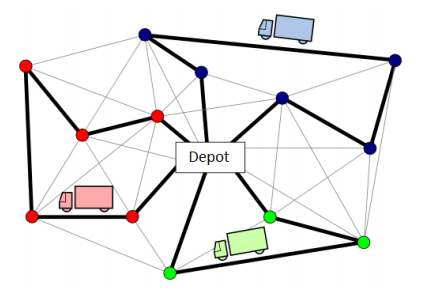
\includegraphics[width=60mm, height=40mm]{cvrp}} \quad\quad
    \subfigure[{ \scriptsize Vehicle Routing Problem, источник - \href{https://en.wikipedia.org/wiki/Vehicle_routing_problem}{Wikipedia}}]{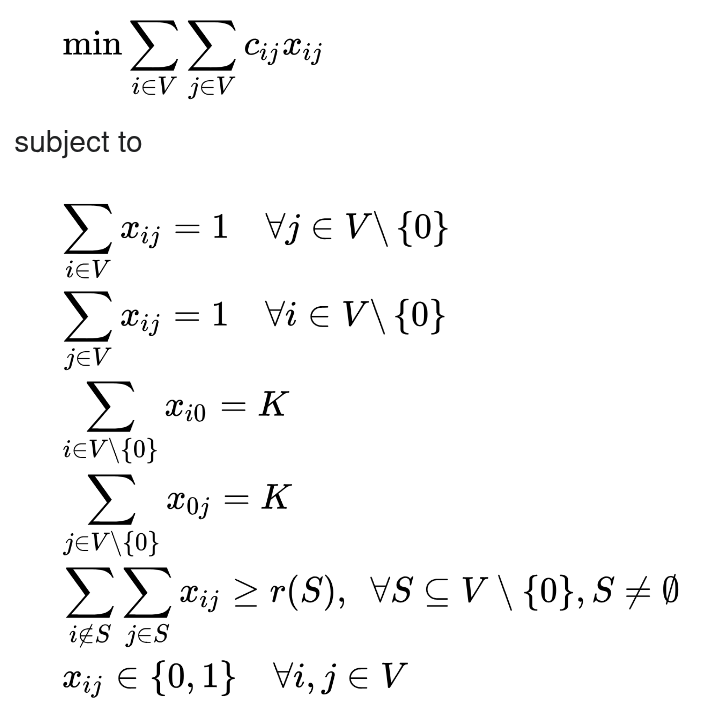
\includegraphics[width=55mm, height=50mm]{cvrp_math}} 
\end{figure}
\end{frame}

%%%%%%%%%%%%%%%%%%%%%%%%%%%%%%%%%%%%%%%%%%%%%%%%%%%%%%%%%%%%%%%%%%%%%%%%%%%%%%%%%%%%%%%%%%%%%%%%%%
\begin{frame}
\frametitle{Вычислительные задачи и корректность алгоритмов}
\framesubtitle{Вычислительные задачи}
\justifying
В современном мире вычислительные задачи возникают практически во все сферы жизни человека, например:
\begin{itemize}
\item{Логистика:  построение маршрутов, оптимизация доставок}
\item{Интернет: организация компьютерных сетей, передача данных, шифрование}
\item{Производство: оптимальное распределение ресурсов}
\item{Искуственный интеллект (AI): алгоримты обучения, сжатия моделей}
\end{itemize}

Как следствие, создание эффективных алгоритмов для решения вычислительных задач становится все более важным направлением.

\end{frame}

%%%%%%%%%%%%%%%%%%%%%%%%%%%%%%%%%%%%%%%%%%%%%%%%%%%%%%%%%%%%%%%%%%%%%%%%%%%%%%%%%%%%%%%%%%%%%%%%%%
\begin{frame}
\frametitle{Вычислительные задачи и корректность алгоритмов}
\framesubtitle{Вычислительные задачи}
\justifying
\small
Алгоритм для решения вычислительной задачи называется \textcolor{red}{правильным (correct)} если для любых возможных входных данных он \textcolor{red}{завершается (halts)} за конечное время и выдает правильный набор выходных данных.\newline\newline
В этом случае говорят, что алгоритм решает задачу. В противном случае алгоритм либо не завершается, либо выдает неверный ответ на один или более наборов входных данных (или даже завершается с ошибкой).\newline\newline
Как правило, корректность алгоритма приходится доказывать математически (для любых возможных наборов входных данных).\newline\newline
Самый простой метод решения задач, почти не требующий доказательств, это \textcolor{red}{метод грубой силы (brute force)} - полный перебор всех вариантов решений.

\end{frame}

%%%%%%%%%%%%%%%%%%%%%%%%%%%%%%%%%%%%%%%%%%%%%%%%%%%%%%%%%%%%%%%%%%%%%%%%%%%%%%%%%%%%%%%%%%%%%%%%%%
\begin{frame}
\frametitle{Вычислительные задачи и корректность алгоритмов}
\framesubtitle{Эвристики и аппроксимационные алгоритмы}
\justifying
\small
В редких случаях некорректные алгоритмы тоже могут быть полезны, например, если они потребляют очень мало вычислительных ресурсов и/или при этом степень ошибки в ответе известна и/или может контролироваться пользователем.\newline\newline
\textcolor{red}{Эвристические алгоритмы (эвристики)} - способны давать хороший результат на практике при умеренном или низком использовании вычислительных ресурсов. Однако, твердых гарантий по качеству решений нет.\newline\newline
\textcolor{red}{Аппроксимационные алгоритмы} - гарантируют качество решения в заявленных границах. Однако, на практике эти границы могут быть весьма широкими.

\end{frame}

%%%%%%%%%%%%%%%%%%%%%%%%%%%%%%%%%%%%%%%%%%%%%%%%%%%%%%%%%%%%%%%%%%%%%%%%%%%%%%%%%%%%%%%%%%%%%%%%%%
\begin{frame}
\frametitle{Массивы, вычислительная сложность, тестирование}
\framesubtitle{План лекции}

\begin{enumerate}
  \setcounter{enumi}{-1}
  \item{План лекции}
  \item{Структура данных массив}
  \item{Вычислительные задачи и корректность алгоритмов}
  \item{\textcolor{blue}{Вычислительная сложность алгоритмов}}
  \item{Тестирование программ}
\end{enumerate}
\end{frame}

%%%%%%%%%%%%%%%%%%%%%%%%%%%%%%%%%%%%%%%%%%%%%%%%%%%%%%%%%%%%%%%%%%%%%%%%%%%%%%%%%%%%%%%%%%%%%%%%%%
\begin{frame}
\frametitle{Вычислительная сложность алгоритмов}
\framesubtitle{Вычислительная сложность}
\justifying
Алгоритм должен быть \textcolor{red}{корректным}, то есть завершаться получением правильного ответа для задачи. Если алгоритм корректен, то имеет смысл говорить о том, насколько \textcolor{red}{эффективно} он использует предоставляемые ему ресурсы. \newline\newline
Алгоритмы обычно оценивают по \textcolor{red}{времени выполнения} и по \textcolor{red}{используемой памяти}. \newline\newline
Такие оценки называют \textcolor{red}{вычислительной сложностью} алгоритма. Чем выше вычисли-тельная сложность, тем дольше работает алгоритм и/или больше памяти использует. \newline\newline
Выделяют два вида вычислительной сложности: \textcolor{red}{временная сложность (time complexity)} и \textcolor{red}{пространственная сложность (space complexity)}.

\end{frame}	

%%%%%%%%%%%%%%%%%%%%%%%%%%%%%%%%%%%%%%%%%%%%%%%%%%%%%%%%%%%%%%%%%%%%%%%%%%%%%%%%%%%%%%%%%%%%%%%%%%
\begin{frame}
\frametitle{Вычислительная сложность алгоритмов}
\framesubtitle{Вычислительная сложность}
\justifying
Фактическое время работы алгоритма зависит от:
\begin{itemize}
\item{скорости работы компьютера}
\item{языка программирования, на котором реализован алгоритм}
\item{компилятора или интерпретатора, который переводит программу в исполняемый код}
\item{опыта разрабатывающего программу программиста}
\item{параллельно выполняемых компьютером задач\newline\newline}
\end{itemize}

Все эти факторы являются внешними по отношению к самому алгоритму.
\end{frame}	

%%%%%%%%%%%%%%%%%%%%%%%%%%%%%%%%%%%%%%%%%%%%%%%%%%%%%%%%%%%%%%%%%%%%%%%%%%%%%%%%%%%%%%%%%%%%%%%%%%
\begin{frame}
\frametitle{Вычислительная сложность алгоритмов}
\framesubtitle{Вычислительная сложность}
\justifying
Как оценить эффективность алгоритма, а не реализации?\newline\newline

\textcolor{blue}{Идея 1}
Привязка оценки эффективности алгоритма к \textcolor{red}{размеру используемых им входных данных} и самим данным.\newline\newline

Объемы данных, обрабатываемых в рамках вычислительных задач, постоянно растут.

\end{frame}	

%%%%%%%%%%%%%%%%%%%%%%%%%%%%%%%%%%%%%%%%%%%%%%%%%%%%%%%%%%%%%%%%%%%%%%%%%%%%%%%%%%%%%%%%%%%%%%%%%%
\begin{frame}
\frametitle{Вычислительная сложность алгоритмов}
\framesubtitle{Вычислительная сложность}
\justifying
Как оценить эффективность алгоритма, а не реализации?\newline\newline

\textcolor{blue}{Идея 2}
Использование  ”элементарных” операций для подсчета времени работы алгоритма.  Элементарными можно считать арифметические операции, ввод-вывод, условный оператор, работу с переменными.

\end{frame}	

%%%%%%%%%%%%%%%%%%%%%%%%%%%%%%%%%%%%%%%%%%%%%%%%%%%%%%%%%%%%%%%%%%%%%%%%%%%%%%%%%%%%%%%%%%%%%%%%%%
\begin{frame}
\frametitle{Вычислительная сложность алгоритмов}
\framesubtitle{Вычислительная сложность}
\justifying
\small
Как оценить эффективность алгоритма, а не реализации?\newline\newline
\textcolor{blue}{Идея 3}
Оценка \textcolor{red}{скорости роста} количества операций при увеличении размера входных данных. Пренебрежение менее значимыми компонентами и константами.\newline\newline
Предположим, мы посчитали все операции, которые производит алгоритм и получили \newline $$T(n) = 5\cdot n^3 + 4\cdot n + 3$$ элементарных операций на входе размера n. \newline Мы можем отбросить слагаемые $4\cdot n$ и $3$, которые при больших n вносят очень маленький вклад в значение функции. \newline Более того, мы можем отбросить и множитель 5 в старшем слагаемом (через несколько лет компьютеры станут в пять раз быстрее) и сказать, что время работы алгоритма растёт также быстро как $n^3$.

\end{frame}

%%%%%%%%%%%%%%%%%%%%%%%%%%%%%%%%%%%%%%%%%%%%%%%%%%%%%%%%%%%%%%%%%%%%%%%%%%%%%%%%%%%%%%%%%%%%%%%%%%
\begin{frame}
\frametitle{Вычислительная сложность алгоритмов}
\framesubtitle{O символика}
\justifying
Пусть даны две функции $f(n)$ и $g(n)$ натурального аргумента $n$, значениями которых являются положительные действительные числа.\newline\newline
Говорят, что $f(n)$ \textcolor{red}{растёт не быстрее} $g(n)$ или $$f(n) = \mathcal{O}(g(n))$$если существует такая константа $c \geq 0$ и число $n_0$, такие что $$f(n) \leq c \cdot g(n) \quad \forall n : n \geq n_0 $$

\end{frame}	

%%%%%%%%%%%%%%%%%%%%%%%%%%%%%%%%%%%%%%%%%%%%%%%%%%%%%%%%%%%%%%%%%%%%%%%%%%%%%%%%%%%%%%%%%%%%%%%%%%
\begin{frame}
\frametitle{Вычислительная сложность алгоритмов}
\framesubtitle{O символика}
\justifying
Пусть имеются два алгоритма: первый выполняет $f(n) = n^2$ операций, а второй $g(n) = 2\cdot n + 20$. Какой из алгоритмов работает быстрее?

\end{frame}

%%%%%%%%%%%%%%%%%%%%%%%%%%%%%%%%%%%%%%%%%%%%%%%%%%%%%%%%%%%%%%%%%%%%%%%%%%%%%%%%%%%%%%%%%%%%%%%%%%
\begin{frame}
\frametitle{Вычислительная сложность алгоритмов}
\framesubtitle{O символика}
\justifying
Пусть имеются два алгоритма: первый выполняет $f(n) = n^2$ операций, а второй $g(n) = 2\cdot n + 20$. Какой из алгоритмов работает быстрее?

\begin{figure}
    \captionsetup[subfigure]{labelformat=empty}
    \centering
    \subfigure[{ \scriptsize Источник - Dasgupta, Papadimitriu, Vazirani}]{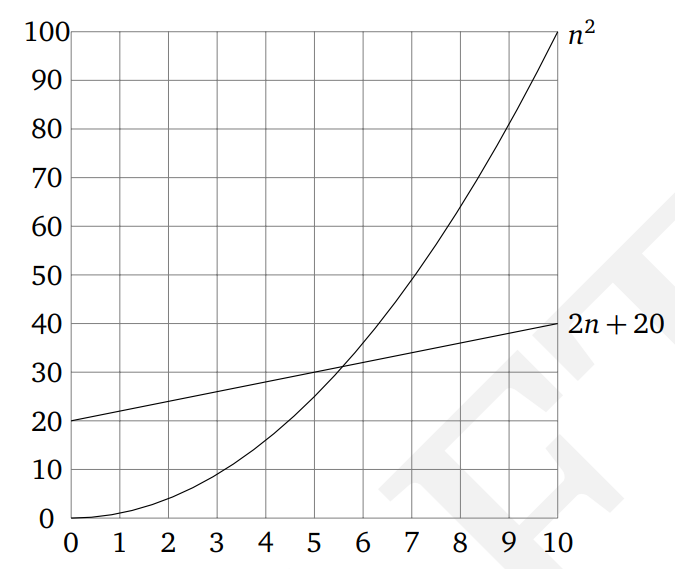
\includegraphics[width=60mm, height=45mm]{bigo_test}} 
\end{figure}
\end{frame}

%%%%%%%%%%%%%%%%%%%%%%%%%%%%%%%%%%%%%%%%%%%%%%%%%%%%%%%%%%%%%%%%%%%%%%%%%%%%%%%%%%%%%%%%%%%%%%%%%%
\begin{frame}
\frametitle{Вычислительная сложность алгоритмов}
\framesubtitle{O символика}
\justifying
Обозначение $f(n) = O(g(n))$ можно считать аналогом математической операции $\leq$. Для операций $\geq$ и $=$ приняты следующие обозначения.\newline\newline

\textcolor{red}{Омега} (большая), $f$ растет не медленнее $g$ с точностью до константы:
$$f(n) = \Omega(g(n))$$\newline
\textcolor{red}{Тета} (большая), $f$ и $g$ имеют одинаковый порядок роста\newline
$$f(n) = \Theta(g(n))$$
\end{frame}

%%%%%%%%%%%%%%%%%%%%%%%%%%%%%%%%%%%%%%%%%%%%%%%%%%%%%%%%%%%%%%%%%%%%%%%%%%%%%%%%%%%%%%%%%%%%%%%%%%
\begin{frame}
\frametitle{Вычислительная сложность алгоритмов}
\framesubtitle{O символика}
\justifying
Несколько правил работы с O символикой

\begin{figure}
    \captionsetup[subfigure]{labelformat=empty}
    \centering
    \subfigure[{ \scriptsize Источник - Dasgupta, Papadimitriu, Vazirani}]{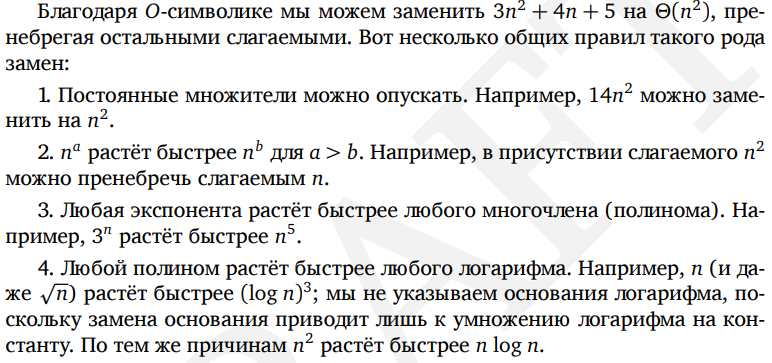
\includegraphics[width=100mm, height=45mm]{bigo_rules}} 
\end{figure}
\end{frame}

%%%%%%%%%%%%%%%%%%%%%%%%%%%%%%%%%%%%%%%%%%%%%%%%%%%%%%%%%%%%%%%%%%%%%%%%%%%%%%%%%%%%%%%%%%%%%%%%%%
\begin{frame}
\frametitle{Вычислительная сложность алгоритмов}
\framesubtitle{Вычислительная сложность}
\justifying

\begin{figure}
    \captionsetup[subfigure]{labelformat=empty}
    \centering
    \subfigure[{ \scriptsize Источник - указать}]{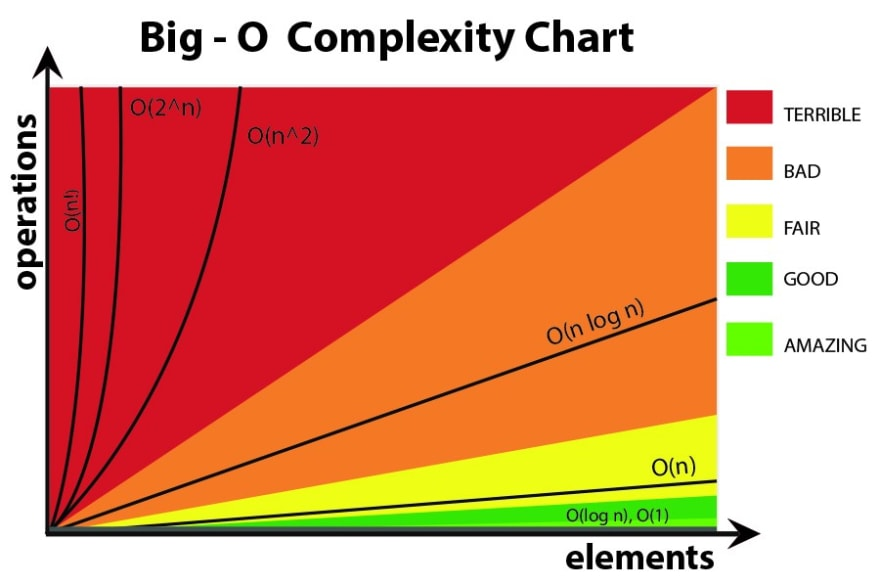
\includegraphics[width=100mm, height=60mm]{bigo_complexity_chart}} 
\end{figure}
\end{frame}

%%%%%%%%%%%%%%%%%%%%%%%%%%%%%%%%%%%%%%%%%%%%%%%%%%%%%%%%%%%%%%%%%%%%%%%%%%%%%%%%%%%%%%%%%%%%%%%%%%
\begin{frame}
\frametitle{Вычислительная сложность алгоритмов}
\framesubtitle{Таблица сложностей}
\justifying

\begin{figure}
    \captionsetup[subfigure]{labelformat=empty}
    \centering
    \subfigure[{ \scriptsize Источник - указать}]{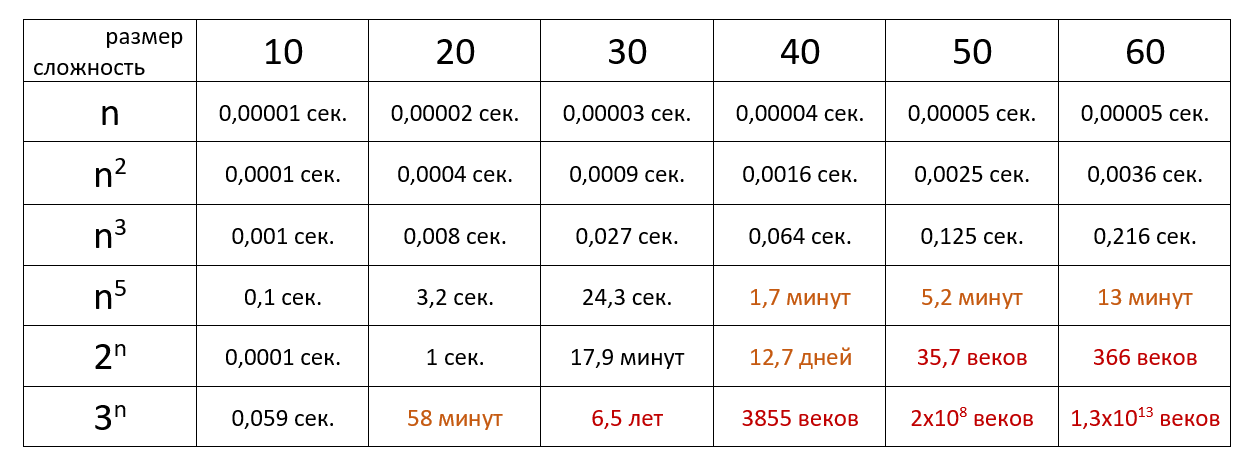
\includegraphics[width=120mm, height=45mm]{complexity_table}} 
\end{figure}
\end{frame}

%%%%%%%%%%%%%%%%%%%%%%%%%%%%%%%%%%%%%%%%%%%%%%%%%%%%%%%%%%%%%%%%%%%%%%%%%%%%%%%%%%%%%%%%%%%%%%%%%%
\begin{frame}
\frametitle{Массивы, вычислительная сложность, тестирование}
\framesubtitle{План лекции}

\begin{enumerate}
  \setcounter{enumi}{-1}
  \item{План лекции}
  \item{Структура данных массив}
  \item{Вычислительные задачи и корректность алгоритмов}
  \item{Вычислительная сложность алгоритмов}
  \item{\textcolor{blue}{Тестирование программ}}
\end{enumerate}
\end{frame}

%%%%%%%%%%%%%%%%%%%%%%%%%%%%%%%%%%%%%%%%%%%%%%%%%%%%%%%%%%%%%%%%%%%%%%%%%%%%%%%%%%%%%%%%%%%%%%%%%%
\begin{frame}
\frametitle{Тестирование программ}
\framesubtitle{Тестирование}
\justifying
\textcolor{red}{Тестирование} программы - процесс проверки программы на наличие ошибок. Состоит в поиске наборов входных данных, на которых поведение алгоритма/программы может отличаться от ожидаемого. \textcolor{red}{Тестирование} и \textcolor{red}{отладка(debugging)} - крайне важные навыки.\newline\newline
Как в алгоритмических соревнованиях, так и в промышленной разработке программ важно последовательно и системно подходить к процессу тестирования.\newline\newline
Проверка алгоритмических задач также основывается на тестировании - тестирующая система подаёт на вход вашей программе различные данные и проверяет правильность ответа.

\end{frame}

%%%%%%%%%%%%%%%%%%%%%%%%%%%%%%%%%%%%%%%%%%%%%%%%%%%%%%%%%%%%%%%%%%%%%%%%%%%%%%%%%%%%%%%%%%%%%%%%%%
\begin{frame}
\frametitle{Тестирование программ}
\framesubtitle{Варианты тестов}
\justifying
\textcolor{red}{Тесты из условия}. Как правило, в условии задач даётся не менее одного примера с входными данными и верным ответом для них. Эти тесты должны быть проверены в первую очередь, с высокой долей вероятности они есть в проверочном наборе. \newline\newline
Более того, на тестах из условия обычно можно проверить формат и вид выводимого ответа. В данном случае нужно быть предельно внимательным - часто даже небольшое отличие (не хватает пробелов между элементами, символы в разных регистрах) может привести к вердикту WRONG ANSWER, даже если по сути ответ правильный.
\begin{figure}
    \captionsetup[subfigure]{labelformat=empty}
    \centering
    \subfigure[{ \scriptsize Источник - указать}]{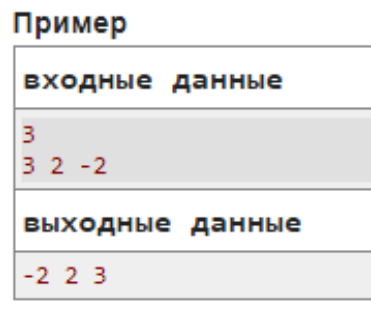
\includegraphics[width=35mm, height=30mm]{testing_statement}} 
\end{figure}
\end{frame}

%%%%%%%%%%%%%%%%%%%%%%%%%%%%%%%%%%%%%%%%%%%%%%%%%%%%%%%%%%%%%%%%%%%%%%%%%%%%%%%%%%%%%%%%%%%%%%%%%%
\begin{frame}
\frametitle{Тестирование программ}
\framesubtitle{Варианты тестов}
\justifying
\textcolor{red}{Тесты наименьшего размера/тривиальные тесты}. \newline Самое простое, что можно проверить самостоятельно - тесты наименьшего размера. Если речь идёт о коллекциях элементов (например, массивах) всегда имеет смысл проверять наименьший возможный размер (конечно, если это предусмотрено интервалами входных параметров). \newline\newline Часто на таких маленьких примерах программы даже ломаются, уходят в бесконечные циклы или даже получают ошибки при обращении к неразрешенному участку памяти. \newline\newline В других случаях, для наименьших тестов может отличаться или не работать логика, корректная для остальных.
\end{frame}


%%%%%%%%%%%%%%%%%%%%%%%%%%%%%%%%%%%%%%%%%%%%%%%%%%%%%%%%%%%%%%%%%%%%%%%%%%%%%%%%%%%%%%%%%%%%%%%%%%
\begin{frame}
\frametitle{Тестирование программ}
\framesubtitle{Варианты тестов}
\justifying
\textcolor{red}{Тесты с наибольшими возможными данными}.\newline Такие тесты обычно содержат граничные допустимые значения переменных задачи. Например, максимально возможное число элементов в соответствии с условием. Или максимально большие значения элементов.\newline\newline
Тесты с наибольшими данными призваны проверить несколько вещей:

\begin{itemize}
\item{укладывается ли предложенный Вами алгоритм в ограничение по времени}
\item{укладывается ли предложенный Вами алгоритм в ограничение по памяти}
\item{правильно ли выбраны типы данных внутри алгоритма, нет ли ошибок переполнения типов}
\end{itemize}

Несмотря на то, что с опытом оценить время и память часто можно без использования дополнительных тестов, иногда бывает необходимо даже написать отдельную программу, которая генерирует большой тест.
\end{frame}

%%%%%%%%%%%%%%%%%%%%%%%%%%%%%%%%%%%%%%%%%%%%%%%%%%%%%%%%%%%%%%%%%%%%%%%%%%%%%%%%%%%%%%%%%%%%%%%%%%
\begin{frame}
\frametitle{Тестирование программ}
\framesubtitle{Варианты тестов}
\justifying
\small
В задаче про суммы максимальными тестами можно считать:
\begin{itemize}
\item{тесты с граничными значениями элементов $a = 10^9$, $a = -10^9$}
\item{тесты массивов с максимальным числом элементов - массив из 500 строк и 500 столбцов}
\item{оба пункта выше одновременно}
\end{itemize}

\begin{figure}
    \captionsetup[subfigure]{labelformat=empty}
    \centering
    \subfigure{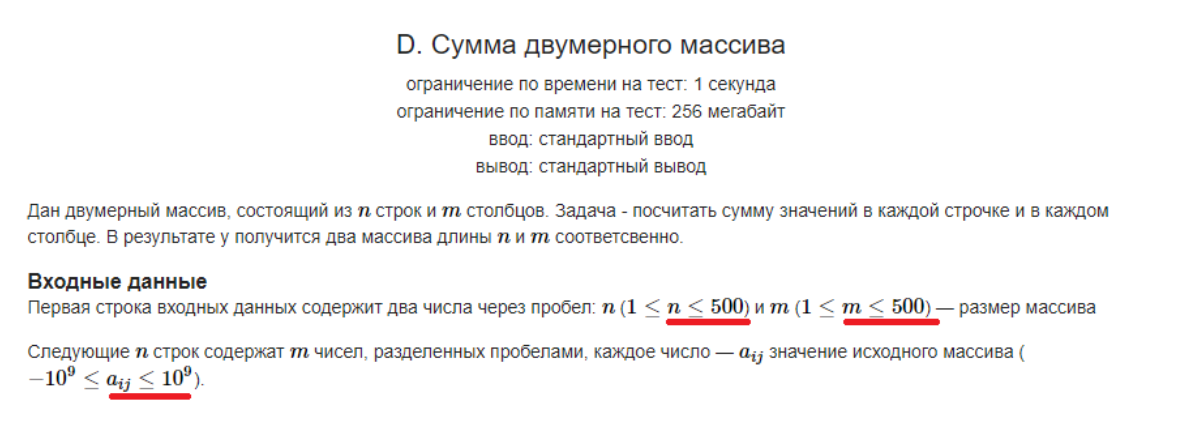
\includegraphics[width=125mm, height=45mm]{testing_max}} 
\end{figure}
\end{frame}

%%%%%%%%%%%%%%%%%%%%%%%%%%%%%%%%%%%%%%%%%%%%%%%%%%%%%%%%%%%%%%%%%%%%%%%%%%%%%%%%%%%%%%%%%%%%%%%%%%
\begin{frame}
\frametitle{Тестирование программ}
\framesubtitle{Варианты тестов}
\justifying
\textcolor{red}{Тесты с различными типами ответов}.\newline Корректному алгоритму почти всегда необходимо по-разному реагировать на различные экземпляры или наборы экземпляров входных данных.\newline\newline
Например, для четного количества элементов массива логика может отличаться (из условия задачи) от логики для нечетного количества элементов.\newline\newline
Или, если речь идет о таком классе задач как игры, на часть примеров нужно будет ответить, например, "Выиграет первый игрок", а на другую "Выиграет второй игрок".\newline\newline
Важно придумать по несколько тестов для каждого возможного варианта ответов (или для каждого возмозного пути выполнения) вашего алгоритма.

\end{frame}



\end{document}